%% Scientific Reports / Springer Nature submission
%% Lesion-guided multi-task learning for renal ultrasound
%%
%% NOTE TO AUTHORS
%%  * Figures 1 and 2 are placeholders awaiting the architecture diagrams.
%%  * Citation keys marked VERIFY in sn-bibliography.bib must be checked before submission.
%%  * Section 2.6 contains a measurement caveat that should be resolved before submission;
%%    see the comment block at that point in the file.

\documentclass[pdflatex,sn-mathphys-num]{sn-jnl}

\usepackage{graphicx}%
\usepackage{multirow}%
\usepackage{amsmath,amssymb,amsfonts}%
\usepackage{amsthm}%
\usepackage{mathrsfs}%
\usepackage[title]{appendix}%
\usepackage{xcolor}%
\usepackage{textcomp}%
\usepackage{manyfoot}%
\usepackage{booktabs}%
\usepackage{algorithm}%
\usepackage{algorithmicx}%
\usepackage{algpseudocode}%
\usepackage{listings}%

\theoremstyle{thmstyleone}%
\newtheorem{theorem}{Theorem}%
\newtheorem{proposition}[theorem]{Proposition}%

\theoremstyle{thmstyletwo}%
\newtheorem{example}{Example}%
\newtheorem{remark}{Remark}%

\theoremstyle{thmstylethree}%
\newtheorem{definition}{Definition}%

\raggedbottom

\begin{document}

\title[Lesion-guided multi-task learning for renal ultrasound]{Lesion-guided multi-task
learning improves kidney disease classification in renal ultrasound}

\author*[1]{\fnm{First} \sur{Author}}\email{iauthor@gmail.com}

\author[1]{\fnm{Second} \sur{Author}}\email{iiauthor@gmail.com}

\author[1]{\fnm{Third} \sur{Author}}\email{iiiauthor@gmail.com}

\affil*[1]{\orgdiv{Department}, \orgname{Organization},
\orgaddress{\street{Street}, \city{City}, \postcode{000000}, \state{State},
\country{Country}}}

%%================================%%
%% Abstract                       %%
%%================================%%

\abstract{Renal ultrasound is the first-line imaging modality for kidney disease, but its
interpretation is operator-dependent and the images are degraded by speckle and low contrast.
Computer-aided diagnosis systems for this modality typically rely on object detectors that
localise findings explicitly, at substantial architectural and computational cost. We present a
single-encoder multi-task network that jointly performs healthy-versus-pathological
classification, multi-label pathology recognition, kidney segmentation and lesion segmentation
from one forward pass, and we show that the classification task benefits materially from being
trained alongside the segmentation tasks: diagnosis AUC rises from 0.8436 when the
classification head is trained alone to 0.8995 within the multi-task model. We further
introduce lesion-guided pooling, in which the lesion segmentation branch is reused as a
detached spatial attention map so that the multi-label pathology classifier reads localised
rather than globally averaged evidence; this improves multi-pathology AUC by 0.0271 under
matched five-fold cross-validation, a result corroborated by an independent three-seed ablation.
Combined with seed ensembling, the final system reaches $0.8969 \pm 0.0155$ AUC for
healthy-versus-pathological classification on the URI-CADS benchmark, exceeding the published
reference value of 0.8741 obtained with a dual-detector architecture using a larger backbone. We
additionally report two negative results that we believe are of practical value: an anatomical
consistency constraint expressed as absolute probability mass is minimised by a degenerate
solution and must be reformulated as a ratio, and three population-based metaheuristics are
statistically indistinguishable from one another at matched evaluation budget.}

\keywords{renal ultrasound, multi-task learning, computer-aided diagnosis, medical image
segmentation, attention mechanisms}

\maketitle

%%================================%%
\section{Introduction}\label{sec:intro}
%%================================%%

Ultrasound is the first-line imaging modality for suspected renal disease. It is inexpensive,
portable, free of ionising radiation, and can be performed at the bedside. These advantages come
at a cost in image quality: B-mode renal ultrasound is corrupted by speckle noise, suffers from
low soft-tissue contrast, and the appearance of a given structure depends strongly on probe
angle, depth setting and operator skill. Interpretation accordingly varies between readers, and
subtle findings such as early loss of corticomedullary differentiation are easily missed. This
interobserver variability is the limitation most often cited as motivating automation in this
modality \cite{bib_renalreview}.

Computer-aided diagnosis (CAD) offers a route to more consistent reading, and deep learning has
become the dominant approach \cite{bib_renalreview}. Most published renal ultrasound CAD systems
fall into one of two families. The first treats the problem as image-level classification,
applying a convolutional backbone to produce a diagnosis or a set of pathology labels. Kuo
\textit{et al.} predicted estimated glomerular filtration rate and chronic kidney disease status
from 4,505 kidney ultrasound images using an ImageNet-pretrained ResNet \cite{bib_kuo2019}, and
convolutional classifiers have since been applied to related image-level decisions such as
selecting the most diagnostically informative frame from an acquisition \cite{bib_frameselect}.
Such systems are simple and fast but provide no spatial evidence for their decisions, which
limits clinical trust and makes errors hard to audit.

A parallel line of work addresses the spatial problem directly through segmentation, delineating
the kidney boundary \cite{bib_shtaiyat,bib_mseunet} or separating multiple renal structures with
attention-augmented networks \cite{bib_renalattn}. These produce localisation but not diagnosis.
A smaller body of work couples the two: Al-Salman and Cevik train a dual-headed network that
performs renal segmentation jointly with functional prediction, tied together by an explicit
structure--function consistency loss \cite{bib_fgckdunet}.

The second family treats the problem as detection or instance segmentation, localising each
finding explicitly with a region-proposal architecture. These systems produce interpretable
output and generally classify better, because a classifier reading a localised region is not
forced to infer a small finding from a whole-image summary. The cost is architectural complexity
and computation: a dual-branch detector with a region proposal network, region-of-interest
pooling and separate mask heads is substantially heavier than a classification backbone, which
matters for deployment on the portable hardware that makes ultrasound attractive in the first
place. Transformer-based alternatives have been explored for ultrasound classification in other
anatomies \cite{bib_fetalvit}, but their data requirements exceed what is available in most
single-institution renal cohorts.

A separate thread applies metaheuristic search to medical imaging pipelines. Most relevant here,
Kausar and Ramamurthy optimise feature selection for kidney ultrasound classification with a
binary Coati algorithm \cite{bib_coatikidney}; comparable hybrid-optimisation pipelines have been
reported for other modalities \cite{bib_dentalopt}. Our use of metaheuristics differs in target:
rather than selecting features for a fixed classifier, we search the multi-task loss weighting
and the image-enhancement parameters jointly, and we report a matched-budget comparison between
optimisers rather than presenting a single algorithm's result.

This work asks whether the localisation advantage of the detection family can be obtained
without adopting a detector. Our starting observation is that a multi-task network performing
segmentation already computes, as one of its outputs, a dense spatial map indicating where the
abnormality lies. That map is ordinarily consumed only by the segmentation loss. We instead reuse
it as a spatial attention map for the classification head, so the pathology classifier reads
features pooled under the model's own predicted lesion distribution in addition to the global
average. The mechanism adds a few thousand parameters and no additional supervision, and it
requires no region proposals, no anchors and no non-maximum suppression. It differs from
gradient-based attribution methods such as CAM and Grad-CAM \cite{bib_cam,bib_gradcam}, which
recover localisation \emph{from} a trained classifier, in that the attention here originates in a
branch supervised independently by its own segmentation target, and from channel-recalibration
attention \cite{bib_senet} in that the weighting is spatial and externally supervised rather than
learned end-to-end from the classification objective alone.

We evaluate on URI-CADS, a public renal ultrasound benchmark of 1,985 images with hand-traced
kidney masks, image-level diagnosis and pathology labels, and bounding-box annotations for local
lesions \cite{bib_uricads}. The benchmark's reference system is a dual architecture combining
Mask R-CNN for the kidney with Faster R-CNN for lesions over a shared ResNet-50 backbone
\cite{bib_maskrcnn,bib_fasterrcnn,bib_resnet}, which places our question in direct form: can a
single ResNet-34 encoder with five lightweight heads match a two-detector system?

Our contributions are as follows.

\begin{enumerate}
\item We quantify the multi-task benefit on this modality under matched conditions, showing that
training the diagnosis head alongside segmentation improves its AUC by 0.056 relative to
single-task training, while the three classification heads together account for under 0.03\% of
model parameters.

\item We introduce lesion-guided pooling, a detached-attention mechanism that reuses the lesion
decoder's own output to localise evidence for the multi-label pathology classifier, and show it
improves multi-pathology AUC by 0.0271 under five-fold cross-validation, corroborated by an
independent three-seed ablation at reduced fidelity.

\item We report a diagnosed negative result with a verified correction. An anatomical
consistency constraint penalising lesion probability outside the kidney \emph{increases} the
violation rate it was intended to reduce, because the absolute-mass formulation admits a
degenerate minimiser; reformulating it as a ratio reduces the violation rate from 0.2331 to
0.0543.

\item We report a second negative result: three population-based metaheuristics applied to loss
weighting and enhancement parameters are statistically indistinguishable at matched evaluation
budget, and none improves classification over equal loss weights.

\item We establish a measurement protocol appropriate to a dataset of this size, quantifying the
seed-induced noise floor and reporting all component claims with error bars and paired tests
against it.
\end{enumerate}

%%================================%%
\section{Results}\label{sec:results}
%%================================%%

\subsection{Dataset and experimental protocol}\label{subsec:data}

The URI-CADS dataset comprises 1,985 B-mode renal ultrasound images. Each image carries a
hand-traced kidney mask, a binary healthy-versus-pathological diagnosis, two whole-organ
pathology labels, and zero or more lesion bounding boxes each tagged with a pathology
identifier. Table~\ref{tab:dataset} gives the composition. The dataset is markedly imbalanced:
1,535 of 1,985 images (77.3\%) are pathological, so a constant ``pathological'' prediction
already achieves 77.3\% accuracy. We therefore report balanced accuracy, sensitivity and
specificity alongside AUC throughout, and tune the decision threshold on validation data rather
than fixing it at 0.5.

\begin{table}[h]
\caption{Composition of the URI-CADS dataset and the splits used in this work}\label{tab:dataset}%
\begin{tabular}{@{}lrrrr@{}}
\toprule
Split & Images & Pathological & Healthy & Share pathological \\
\midrule
Train       & 1{,}389 & 1{,}074 & 315 & 77.3\% \\
Validation  &    298  &    231  &  67 & 77.5\% \\
Test        &    298  &    230  &  68 & 77.2\% \\
\midrule
Total       & 1{,}985 & 1{,}535 & 450 & 77.3\% \\
\botrule
\end{tabular}
\footnotetext{1,323 of 1,985 images (66.6\%) contain at least one annotated lesion bounding box.
The held-out test split contains 203 lesion-bearing images.}
\end{table}

Unless otherwise stated, models are trained at $512 \times 512$ resolution for 15 epochs with
Adam \cite{bib_adam} at learning rate $10^{-4}$, batch size 4 and mixed precision, on a single
NVIDIA RTX 3050 laptop GPU. Augmentation is geometric only; the rationale is given in
Section~\ref{subsec:augmentation}. All comparisons that support a claim in this paper are run
under matched five-fold cross-validation, the protocol used by the reference system, so that
fold difficulty is averaged out rather than confounded with the comparison.

\subsection{The noise floor of this dataset}\label{subsec:noise}

Before reporting any comparison we quantify how much of an observed difference could arise from
training stochasticity alone. Retraining an identical configuration with different random seeds
moves diagnosis AUC by a standard deviation of 0.0258, with an observed range of 0.074 across
five seeds. On a dataset of this size, therefore, a single-split AUC difference below roughly
0.03 carries no information. This figure governs the interpretation of every result that
follows, and we report it explicitly because several differences we measured fall below it and
are consequently reported as null rather than as findings.

\subsection{Architecture}\label{subsec:architecture}

The network consists of one shared encoder feeding five task-specific heads
(Fig.~\ref{fig:architecture}). A ResNet-34 backbone pretrained on ImageNet, with its classifier
and global pooling removed, maps the $512 \times 512 \times 3$ input to a $512 \times 16 \times
16$ feature map. Global average pooling reduces this to a 512-dimensional vector that feeds three
linear classification heads: one logit for the binary diagnosis, two for whole-organ pathologies
and nine for local pathology types. Two independent decoders consume the full spatial feature map
and upsample it back to input resolution, producing dense logits for the kidney mask and the
lesion region respectively. Each decoder comprises five blocks of $3\times3$ convolution, batch
normalisation \cite{bib_batchnorm}, ReLU and bilinear $2\times$ upsampling, halving the channel count at each stage,
followed by a $1\times1$ convolution to a single output channel.

%%%%%%%%%%%%%%%%%%%%%%%%%%%%%%%%%%%%%%%%%%%%%%%%%%%%%%%%%%%%%%%%%%%%%%%%
%% PLACEHOLDER - Figure 1: overall architecture diagram               %%
%% Should show: input image -> ResNet-34 encoder -> (a) global average %%
%% pooling -> 3 linear heads; (b) full feature map -> 2 decoders.      %%
%% Mark the encoder as shared. Indicate tensor shapes at each stage.   %%
%%%%%%%%%%%%%%%%%%%%%%%%%%%%%%%%%%%%%%%%%%%%%%%%%%%%%%%%%%%%%%%%%%%%%%%%
\begin{figure}[h]
\centering
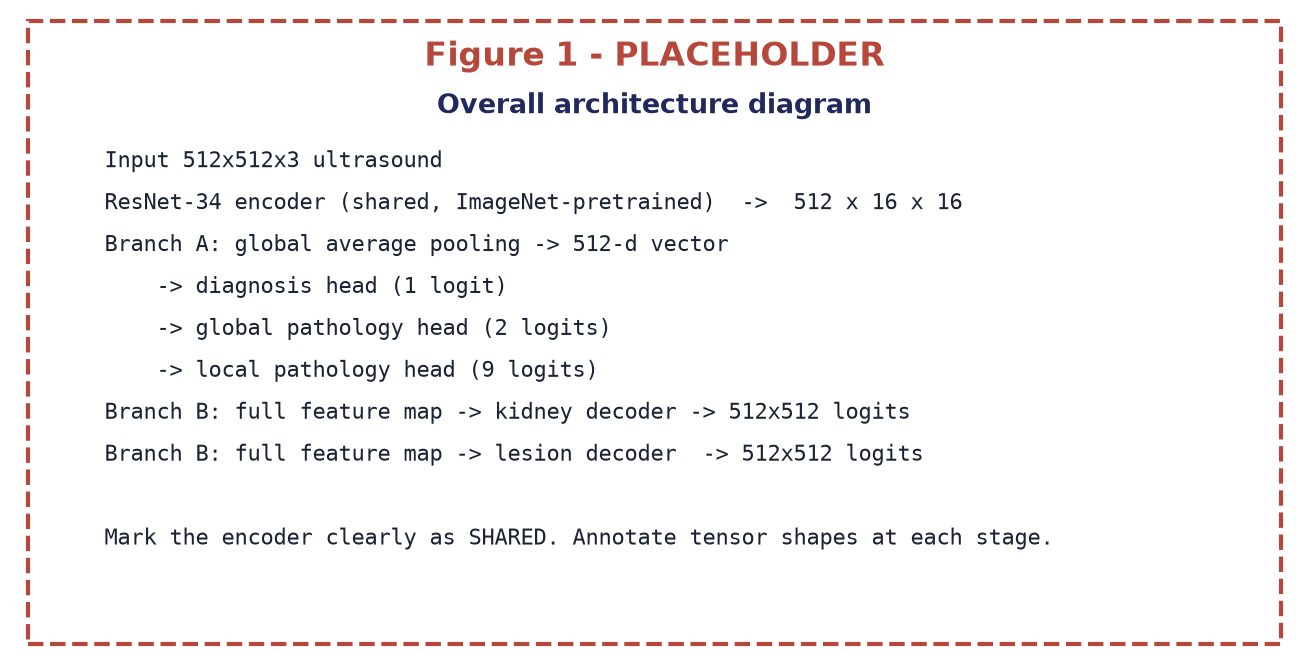
\includegraphics[width=0.95\textwidth]{fig1_architecture}
\caption{Overall architecture of the proposed multi-task network. A single ResNet-34 encoder
produces a shared feature representation consumed by five heads: three linear classifiers
operating on the globally pooled vector, and two convolutional decoders operating on the full
spatial feature map. \textbf{[PLACEHOLDER - diagram to be supplied]}}\label{fig:architecture}
\end{figure}

The parameter budget is strongly dominated by the shared components. The encoder accounts for
21,284,672 parameters and the two decoders for 1,572,833 each, against 6,156 for all three
classification heads combined --- under 0.03\% of the 24.4 M total. The classification outputs
are therefore close to free once the segmentation network exists, which is the efficiency
argument for the multi-task design.

\subsection{Multi-task training improves classification}\label{subsec:multitask}

To isolate the contribution of multi-task learning we trained each task in isolation under
otherwise identical conditions and compared against the joint model
(Table~\ref{tab:singletask}). The diagnosis head trained alone reaches 0.8436 AUC; the same head
inside the multi-task model reaches 0.8995, an improvement of 0.0559 that is more than twice the
noise floor established in Section~\ref{subsec:noise}. The segmentation tasks act as a
regulariser on the shared encoder, forcing it to retain spatial structure that a
classification-only objective would discard, which is the mechanism originally proposed for
multi-task learning \cite{bib_caruana}.

The benefit is not symmetric. Kidney segmentation trained alone reaches 0.9162 Dice against
0.8928 in the joint model, so segmentation pays a modest price for sharing capacity with the
classification objectives. The trade is favourable overall, but it should be reported as a trade
rather than as a uniform gain.

\begin{table}[h]
\caption{Single-task versus multi-task training. Each single-task model is trained with only the
indicated loss term active, all other settings held fixed}\label{tab:singletask}%
\begin{tabular*}{\textwidth}{@{\extracolsep\fill}lcccc}
\toprule
Configuration & Diagnosis & Multi-pathology & Kidney & Lesion Dice \\
              & AUC       & AUC             & Dice   & (lesion-bearing) \\
\midrule
Diagnosis only              & 0.8436 & 0.4040 & 0.1270 & 0.0237 \\
Kidney segmentation only    & 0.5711 & 0.4542 & \textbf{0.9162} & 0.0197 \\
Lesion segmentation only    & 0.4573 & 0.4748 & 0.0967 & 0.4960 \\
\midrule
Multi-task (all five heads) & \textbf{0.8995} & \textbf{0.7704} & 0.8928 & \textbf{0.5056} \\
\botrule
\end{tabular*}
\footnotetext{Values for tasks without a corresponding head reflect an untrained output and are
reported only to confirm that the single-task models carry no incidental ability on the tasks
they were not trained for.}
\end{table}

\subsection{Lesion-guided pooling}\label{subsec:pooling}

Global average pooling summarises the entire image in one vector. For a binary
healthy-versus-pathological decision this is adequate, since diffuse changes affect the whole
organ. For multi-label pathology recognition it is a structural disadvantage: a focal lesion
occupying a small fraction of the field is averaged together with a large volume of normal
tissue before the classifier sees it. This is the most plausible explanation for the one metric
on which our baseline clearly trailed the reference system, which localises each finding
explicitly before classifying it.

Lesion-guided pooling addresses this without introducing a detector
(Fig.~\ref{fig:pooling}). Let $\mathbf{F} \in \mathbb{R}^{C \times H \times W}$ be the encoder
feature map and $\mathbf{L} \in \mathbb{R}^{H' \times W'}$ the lesion decoder's output logits.
We form an attention map

\begin{equation}
\mathbf{A} = \frac{\phi\!\left(\sigma(\mathbf{L})\right)}
                  {\sum_{h,w} \phi\!\left(\sigma(\mathbf{L})\right)_{h,w} + \epsilon},
\label{eq:attention}
\end{equation}

where $\sigma$ is the logistic function, $\phi$ denotes adaptive average pooling to the
encoder's spatial resolution, and $\epsilon$ guards against division by zero. The
lesion-focused descriptor is then

\begin{equation}
\mathbf{v}_{\text{lesion}} = \sum_{h,w} \mathbf{A}_{h,w}\, \mathbf{F}_{:,h,w},
\label{eq:lesionvec}
\end{equation}

and the multi-label pathology head classifies from
$[\mathbf{v}_{\text{global}} \,\Vert\, \mathbf{v}_{\text{lesion}}]$, the concatenation of the
ordinary globally averaged descriptor with the lesion-focused one.

\textbf{The attention map is detached from the computation graph.} This is the critical design
decision. Were gradients allowed to flow from the pathology classification loss back into the
lesion decoder, that loss could reshape the lesion decoder to make classification easier ---
producing convenient pseudo-lesions that improve the classifier while degrading the
segmentation output the clinician actually sees. Detaching makes the attention read-only: the
lesion decoder remains supervised solely by its own Dice term, and lesion-guided pooling can
only exploit localisation the decoder has already learned for its own sake.

%%%%%%%%%%%%%%%%%%%%%%%%%%%%%%%%%%%%%%%%%%%%%%%%%%%%%%%%%%%%%%%%%%%%%%%%
%% PLACEHOLDER - Figure 2: lesion-guided pooling detail                %%
%% Should show: encoder feature map, lesion decoder output, sigmoid,   %%
%% STOP-GRADIENT marker, downsample, normalise, weighted sum, concat   %%
%% with global average vector, into the local-pathology head.          %%
%% The stop-gradient should be visually prominent.                     %%
%%%%%%%%%%%%%%%%%%%%%%%%%%%%%%%%%%%%%%%%%%%%%%%%%%%%%%%%%%%%%%%%%%%%%%%%
\begin{figure}[h]
\centering
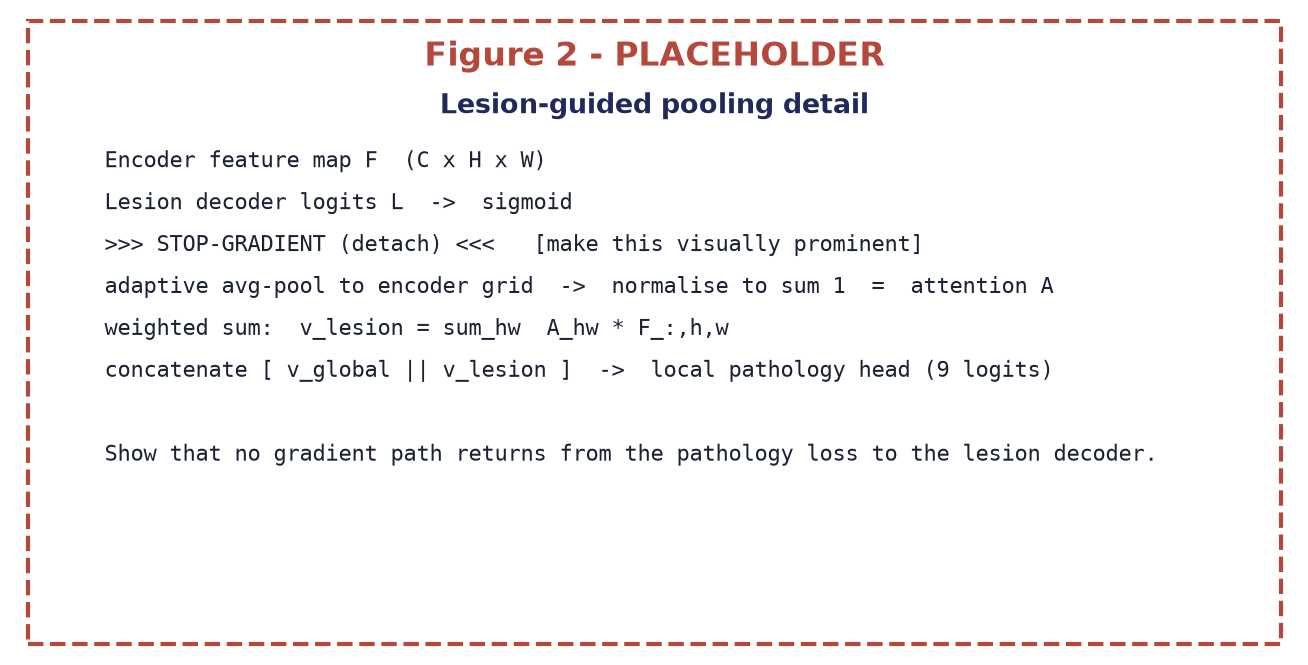
\includegraphics[width=0.9\textwidth]{fig2_lesion_guided_pooling}
\caption{Lesion-guided pooling. The lesion decoder's predicted probability map is detached,
resampled to the encoder grid and normalised to form spatial attention weights, which produce a
lesion-focused feature vector. This is concatenated with the conventional globally averaged
vector before multi-label pathology classification. The stop-gradient prevents the
classification loss from reshaping the segmentation output.
\textbf{[PLACEHOLDER - diagram to be supplied]}}\label{fig:pooling}
\end{figure}

Under matched five-fold cross-validation, lesion-guided pooling raises multi-pathology AUC from
$0.7510 \pm 0.0240$ to $0.7781 \pm 0.0131$, an improvement of 0.0271
(Table~\ref{tab:crossval}). An independent ablation at reduced fidelity with three random seeds,
described in Section~\ref{subsec:ablation}, found a decrease of 0.0428 when the component was
removed, with all three seeds agreeing in direction. Two protocols differing in resolution,
epoch count, split strategy and seed thus agree on both the sign and the approximate magnitude
of the effect.

\subsection{Comparison with the reference system}\label{subsec:benchmark}

Table~\ref{tab:crossval} reports the full cross-validated comparison. The addition of seed
ensembling \cite{bib_ensembles} --- averaging predicted probabilities across three models
trained with different seeds --- lifts diagnosis AUC to $0.8969 \pm 0.0155$, exceeding the reference system's published
0.8741 by 0.0228 while using a ResNet-34 encoder against the reference's ResNet-50 and a single
forward pass against a dual-detector pipeline.

\begin{table}[h]
\caption{Five-fold cross-validated comparison. Values are mean $\pm$ standard deviation across
folds}\label{tab:crossval}%
\begin{tabular*}{\textwidth}{@{\extracolsep\fill}lcccc}
\toprule
System & Diagnosis & Balanced & Multi-pathology & Kidney \\
       & AUC       & accuracy & AUC             & Dice \\
\midrule
Baseline multi-task          & $0.8619 \pm 0.0190$ & $0.7204 \pm 0.0283$
                             & $0.7510 \pm 0.0240$ & $\mathbf{0.8948 \pm 0.0053}$ \\
\quad + lesion-guided pooling & $0.8574 \pm 0.0202$ & $0.7087 \pm 0.0558$
                             & $0.7781 \pm 0.0131$ & $0.8919 \pm 0.0040$ \\
\quad + seed ensemble (final) & $\mathbf{0.8969 \pm 0.0155}$ & $\mathbf{0.7246 \pm 0.0448}$
                             & $\mathbf{0.7883 \pm 0.0258}$ & $0.8893 \pm 0.0068$ \\
\midrule
Reference system \cite{bib_uricads} & 0.8741 & --- & 0.8190 & --- \\
\botrule
\end{tabular*}
\footnotetext{The reference system is a dual Mask R-CNN / Faster R-CNN architecture over a
shared ResNet-50 backbone, evaluated under five-fold cross-validation on the same dataset.}
\end{table}

Multi-pathology AUC reaches $0.7883 \pm 0.0258$ against the reference's 0.8190.

%%%%%%%%%%%%%%%%%%%%%%%%%%%%%%%%%%%%%%%%%%%%%%%%%%%%%%%%%%%%%%%%%%%%%%%%
%% AUTHOR ACTION REQUIRED BEFORE SUBMISSION                            %%
%% The multi-pathology comparison above is NOT yet like-for-like. Our  %%
%% model is trained on the nine raw annotation identifiers; the        %%
%% reference groups them into four lesion classes plus two global      %%
%% pathologies before training (raw 2,3 -> cyst; 4 -> pyramids;        %%
%% 7 -> hydronephrosis; 1,5,6,8,9 -> others). Averaging AUC over nine  %%
%% raw classes includes classes with 11, 33 and 38 positive images,    %%
%% which depresses the mean relative to the grouped taxonomy.          %%
%% Either (a) recompute under the grouped taxonomy, or (b) retrain     %%
%% with grouped labels, before this number is reported as a deficit.   %%
%% The paragraph below is written to be honest under the current state %%
%% and should be replaced once the comparable number is available.     %%
%%%%%%%%%%%%%%%%%%%%%%%%%%%%%%%%%%%%%%%%%%%%%%%%%%%%%%%%%%%%%%%%%%%%%%%%

We draw attention to a caveat affecting this particular comparison. Our model predicts the nine
raw lesion identifiers present in the annotation files, whereas the reference system groups
these into four consolidated lesion classes before training, merging five sparsely populated
identifiers into a single ``others'' category. Three of our nine classes have fewer than 40
positive images in the entire dataset, and averaging per-class AUC over such classes depresses
the mean relative to the grouped taxonomy. The two multi-pathology figures are therefore not
measured on an identical label space, and the apparent deficit should be interpreted with
caution pending evaluation under the matched taxonomy.

Table~\ref{tab:crossval} also shows that the binary classification gain comes from ensembling
rather than from lesion-guided pooling, which is specific to the multi-label task and slightly
negative on the binary task --- within the noise floor, but we do not claim a binary improvement
for it. Sensitivity and specificity for the final system are $0.9336 \pm 0.0387$ and $0.5156
\pm 0.1232$ respectively, reflecting the prevalence of the dataset; the operating point is
tunable and should be selected according to the relative cost of missed disease versus false
alarm in the intended deployment.

\subsection{Anatomical consistency: a negative result and its correction}\label{subsec:consistency}

A lesion within a kidney cannot lie outside the kidney. We encoded this as an auxiliary loss
penalising predicted lesion probability falling outside the annotated kidney region, and
reported a violation rate defined as the fraction of predicted lesion probability mass lying
outside the kidney,

\begin{equation}
R = \frac{\sum_{h,w} \sigma(\mathbf{L})_{h,w}\,(1 - \mathbf{K}_{h,w})}
         {\sum_{h,w} \sigma(\mathbf{L})_{h,w} + \epsilon},
\label{eq:violation}
\end{equation}

with $\mathbf{K}$ the ground-truth kidney mask. The constraint was initially written as the
absolute outside mass,

\begin{equation}
\mathcal{L}_{\text{abs}} = \frac{1}{HW}\sum_{h,w}
      \sigma(\mathbf{L})_{h,w}\,(1 - \mathbf{K}_{h,w}).
\label{eq:consabs}
\end{equation}

Measured against an unconstrained baseline, this constraint made the violation rate
\emph{worse}, rising from 0.2331 to 0.2817 (Table~\ref{tab:consistency}). The cause is that
Eq.~\eqref{eq:consabs} and Eq.~\eqref{eq:violation} are not the same objective.
Eq.~\eqref{eq:consabs} is minimised by suppressing $\sigma(\mathbf{L})$ everywhere, which
shrinks the numerator and denominator of Eq.~\eqref{eq:violation} together and leaves the ratio
unchanged while reducing the loss. The optimiser found this degenerate solution.

Reformulating the constraint as the ratio itself,

\begin{equation}
\mathcal{L}_{\text{ratio}} = \frac{1}{N}\sum_{n=1}^{N}
   \frac{\sum_{h,w} \sigma(\mathbf{L}^{(n)})_{h,w}\,(1 - \mathbf{K}^{(n)}_{h,w})}
        {\sum_{h,w} \sigma(\mathbf{L}^{(n)})_{h,w} + \epsilon},
\label{eq:consratio}
\end{equation}

removes the degenerate minimiser, because a global rescaling of lesion probability leaves a
ratio invariant and the only remaining way to reduce the loss is to move probability mass inside
the kidney. The corrected constraint reduces the violation rate to 0.0543, a factor of roughly
four below the unconstrained baseline.

\begin{table}[h]
\caption{Effect of the anatomical consistency constraint formulation}\label{tab:consistency}%
\begin{tabular*}{\textwidth}{@{\extracolsep\fill}lcccc}
\toprule
Configuration & Violation rate & Diagnosis AUC & Kidney Dice & Lesion Dice \\
              & (lower better) &               &             & (lesion-bearing) \\
\midrule
No constraint                      & 0.2331 & 0.8995 & 0.8928 & 0.5056 \\
Absolute-mass constraint, Eq.~\eqref{eq:consabs}
                                   & 0.2817 & 0.8791 & 0.8838 & 0.4868 \\
Ratio constraint, Eq.~\eqref{eq:consratio}
                                   & \textbf{0.0543} & 0.9014 & 0.8954 & 0.4881 \\
\botrule
\end{tabular*}
\footnotetext{Single held-out split. Differences in the diagnosis AUC column fall within the
noise floor of 0.0258 established in Section~\ref{subsec:noise} and are not interpreted; the
violation rate differences are an order of magnitude larger.}
\end{table}

We report this because the failure mode is general. Any auxiliary constraint written as a
surrogate for a reported ratio metric is vulnerable to the same degeneracy, and the symptom ---
a constraint that worsens the quantity it targets --- is only visible if that quantity is
measured before and after the constraint is introduced.

\subsection{Ablation of model components}\label{subsec:ablation}

We ablated each component in turn with three random seeds per configuration at reduced fidelity
($256 \times 256$, 12 epochs), reporting mean $\pm$ standard deviation
(Table~\ref{tab:ablation}). With three seeds this study detects large effects only; a null
result indicates that an effect was not demonstrated, not that it is absent.

No removal moved diagnosis AUC beyond the noise band. The only component with a demonstrable
effect is lesion-guided pooling, and only on the multi-label task, where removal costs 0.0428
AUC with all three seeds agreeing in direction. Removal of the lesion decoder, which also
removes lesion-guided pooling and the consistency term since both depend on it, costs 0.0282.

\begin{table}[h]
\caption{Component ablation. Three seeds per configuration at reduced fidelity}\label{tab:ablation}%
\begin{tabular*}{\textwidth}{@{\extracolsep\fill}lccc}
\toprule
Configuration & Diagnosis AUC & Multi-pathology AUC & Kidney Dice \\
\midrule
Full model (reference)       & $0.8607 \pm 0.0399$ & $\mathbf{0.8105 \pm 0.0037}$ & $0.8116 \pm 0.0384$ \\
Without lesion-guided pooling & $0.8813 \pm 0.0080$ & $0.7677 \pm 0.0211$ & $0.7621 \pm 0.0395$ \\
Without anatomical consistency & $0.8825 \pm 0.0143$ & $0.7903 \pm 0.0311$ & $0.8048 \pm 0.0096$ \\
Without lesion segmentation   & $0.8728 \pm 0.0270$ & $0.7823 \pm 0.0206$ & $0.7546 \pm 0.0485$ \\
Without kidney segmentation   & $0.8848 \pm 0.0129$ & $0.7997 \pm 0.0202$ & --- \\
Classification heads only     & $0.8649 \pm 0.0051$ & $0.7906 \pm 0.0110$ & --- \\
\botrule
\end{tabular*}
\footnotetext{The reduced-fidelity protocol yields lower absolute values than the main
experiments and the rows should be compared only with one another. The full model's elevated
seed variance in the diagnosis column is driven by one outlying run.}
\end{table}

\subsection{Encoder comparison}\label{subsec:encoders}

We replaced the ResNet-34 backbone with three lighter alternatives under the same protocol
(Table~\ref{tab:encoders}). EfficientNet-B0 \cite{bib_efficientnet} matches ResNet-34 on binary
diagnosis within the noise band using 2.3 times fewer parameters. All three lightweight
backbones, however, lose multi-pathology AUC, by 0.053 to 0.094. The practical reading is that a
smaller backbone is defensible if binary triage is the deployment target, but not if multi-label
pathology recognition is required.

\begin{table}[h]
\caption{Encoder comparison. Three seeds per configuration at reduced fidelity}\label{tab:encoders}%
\begin{tabular*}{\textwidth}{@{\extracolsep\fill}lrcc}
\toprule
Encoder & Parameters & Diagnosis AUC & Multi-pathology AUC \\
\midrule
ResNet-34 \cite{bib_resnet}            & 24.44 M & $\mathbf{0.8607 \pm 0.0399}$ & $\mathbf{0.8105 \pm 0.0037}$ \\
EfficientNet-B0 \cite{bib_efficientnet} & 10.72 M & $0.8569 \pm 0.0136$ & $0.7576 \pm 0.0366$ \\
MobileNetV3-Large \cite{bib_mobilenet}  &  8.20 M & $0.8248 \pm 0.0232$ & $0.7211 \pm 0.0170$ \\
ShuffleNetV2 \cite{bib_shufflenet}      &  6.78 M & $0.8321 \pm 0.0049$ & $0.7169 \pm 0.0181$ \\
\botrule
\end{tabular*}
\footnotetext{Parameter counts are for the complete multi-task model including both decoders and
all heads. Inference latency was not measured and no deployment claim is made on the basis of
parameter count alone.}
\end{table}

\subsection{Metaheuristic optimisation of loss weights and enhancement}\label{subsec:optim}

The loss weights and the image-enhancement parameters are free hyperparameters that prior phases
set by convention: unit weights and fixed contrast-limited adaptive histogram equalisation
(CLAHE) settings. We searched the joint ten-dimensional space --- six loss weights in $[0.1,
5.0]$ and four enhancement parameters --- with three population-based metaheuristics: the Coati
Optimization Algorithm \cite{bib_coa}, the Whale Optimization Algorithm \cite{bib_woa} and the
Grey Wolf Optimizer \cite{bib_gwo}. Each was given an identical budget of 60 fitness
evaluations, where one evaluation trains a model from scratch at reduced fidelity. Equal budget
rather than equal iteration count is the fair basis of comparison, since the algorithms use
different population sizes.

The three optimisers finished within 0.0097 fitness of one another
(Table~\ref{tab:optimizers}), far below this pipeline's run-to-run variation. We therefore
report no meaningful difference between them. More importantly, the optimised configuration did
not improve classification over equal loss weights: it improved kidney Dice to 0.9081 and
reduced the violation rate roughly fivefold, while diagnosis AUC fell to 0.8753. This is
consistent with the fitness function, which placed half its weight on the two segmentation
terms; the search traded classification for segmentation exactly as instructed. We report this
as a negative result for the optimisation framing rather than presenting the winning optimiser
as a contribution.

\begin{table}[h]
\caption{Metaheuristic comparison at matched budget of 60 fitness evaluations}\label{tab:optimizers}%
\begin{tabular}{@{}lccc@{}}
\toprule
Optimiser & Best validation fitness & Evaluations & Wall clock \\
\midrule
Coati Optimization Algorithm \cite{bib_coa} & 0.6080 & 60 & 1.97 h \\
Grey Wolf Optimizer \cite{bib_gwo}          & 0.6006 & 60 & 1.94 h \\
Whale Optimization Algorithm \cite{bib_woa} & 0.5983 & 60 & 1.73 h \\
\botrule
\end{tabular}
\footnotetext{Fitness is the weighted validation score defined in Eq.~\eqref{eq:fitness}. The
spread across the three optimisers is 0.0097.}
\end{table}

\subsection{Qualitative results}\label{subsec:qualitative}

Fig.~\ref{fig:qualitative} shows predictions on held-out test images. The kidney boundary is
recovered closely in both the unenhanced and enhanced input conditions. Lesion predictions are
correctly localised but organically shaped, whereas the ground truth is rectangular by
construction, which is discussed in Section~\ref{subsec:limitations}.

\begin{figure}[h]
\centering
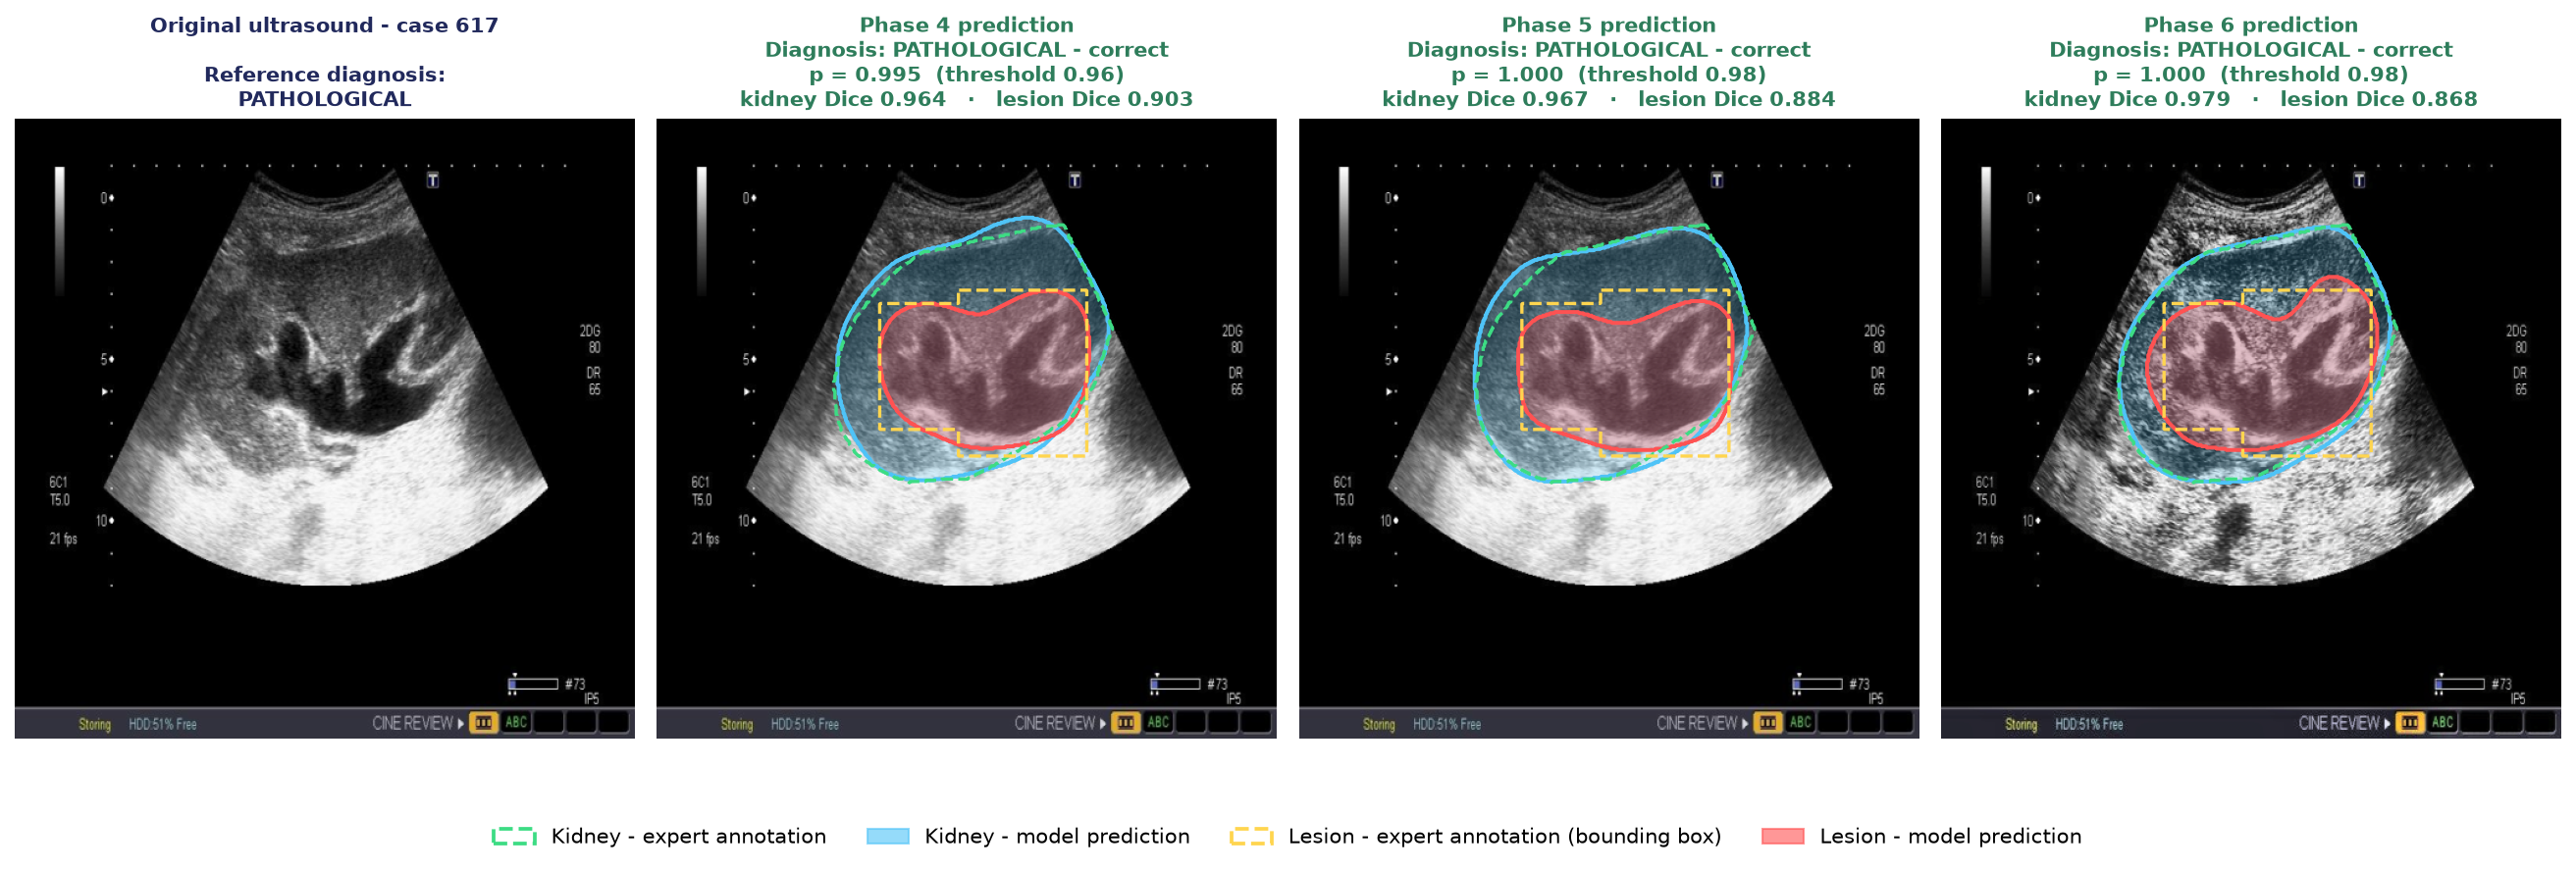
\includegraphics[width=\textwidth]{fig3_qualitative}
\caption{Qualitative results on held-out test cases. Left to right: original ultrasound,
followed by predictions from successive model configurations. Dashed contours denote expert
annotation, filled regions with solid contours denote model prediction; green and blue mark the
kidney, yellow and red the lesion. Each panel reports the classification decision at the
validation-tuned operating point together with per-case Dice.}\label{fig:qualitative}
\end{figure}

%%================================%%
\section{Discussion}\label{sec:discussion}
%%================================%%

The central finding of this work is that the localisation advantage normally obtained by
adopting a detection architecture can be partially recovered within a multi-task segmentation
network at negligible parameter cost. Lesion-guided pooling adds 4,608 parameters --- a widening
of one linear layer --- and no new supervision, yet improves multi-label pathology recognition by
0.0271 AUC under cross-validation. The mechanism is available to any multi-task network that
already segments the structure of interest, and it does not require the region proposals,
anchors or non-maximum suppression that make detector pipelines costly.

The decision to detach the attention map deserves emphasis because it is easy to omit and its
consequences are not visible in classification metrics. An attached attention map would allow
the classification objective to optimise the segmentation output for its own convenience; the
classifier might improve while the lesion mask shown to a clinician degrades. In a diagnostic
setting where the segmentation output is itself part of the deliverable, this coupling is
unacceptable, and detaching costs nothing.

This also distinguishes the mechanism from the two established routes to spatial attention in
this area. Attention modules placed inside a renal segmentation network \cite{bib_renalattn}
refine that network's own output but do not feed a diagnostic classifier. Attribution methods
such as CAM and Grad-CAM \cite{bib_cam,bib_gradcam} run in the opposite direction, recovering a
localisation map from an already-trained classifier, so the map inherits whatever the classifier
happened to rely on. Lesion-guided pooling instead takes a map that was supervised against
annotated lesions and hands it to the classifier, which is why the stop-gradient is both possible
and necessary.

A similar instinct motivates the structure--function consistency loss of Al-Salman and Cevik
\cite{bib_fgckdunet}, which likewise couples a segmentation branch to a second task in a renal
network. Their coupling runs between two predictive heads; ours constrains a single head against
an anatomical prior, and our results in Section~\ref{subsec:consistency} suggest such couplings
need their target metric measured explicitly before and after, since the obvious formulation can
fail silently.

Our binary classification result exceeds the published reference despite a smaller backbone and
a single-pass architecture. We attribute the margin primarily to seed ensembling, which lifted
AUC by 0.0395 over the single V3 model --- larger than any architectural change we tested. This
is worth stating plainly: on a dataset of fewer than 2,000 images, variance reduction is a more
effective lever than architectural refinement, and much of the published variation between
methods at this scale may be seed variance rather than method difference. The noise-floor
measurement in Section~\ref{subsec:noise} is, in our view, the methodological contribution most
transferable to other work on datasets of this size.

The multi-pathology task remains the weaker side of our results, and the taxonomy caveat in
Section~\ref{subsec:benchmark} means we cannot presently state the size of the gap with
confidence. Independently of that measurement issue, the reference architecture retains a
genuine structural advantage: it classifies each detected region separately, whereas our
pathology head must represent an arbitrary number of findings of different types in a single
pair of pooled vectors. Lesion-guided pooling narrows this gap but does not close it, since one
attention map cannot separate two lesions of different types in the same image.

Two negative results are reported here deliberately. The anatomical consistency failure
(Section~\ref{subsec:consistency}) illustrates a general hazard in constrained medical imaging
objectives: a surrogate loss that merely correlates with the reported metric may admit a
minimiser that improves the loss while worsening the metric. Detecting this required measuring
the violation rate both with and without the constraint, which is not standard practice. The
metaheuristic result (Section~\ref{subsec:optim}) is reported because the literature applying
nature-inspired optimisers to deep learning hyperparameters rarely includes a matched-budget
comparison between optimisers or against simple baselines \cite{bib_randomsearch}; our finding
that three such algorithms are indistinguishable at 60 evaluations suggests that reported
differences between them may not survive such a control.

This bears directly on the closest prior work. Kausar and Ramamurthy report gains from a binary
Coati algorithm applied to feature selection for kidney ultrasound classification
\cite{bib_coatikidney}, and hybrid-optimisation pipelines are reported to help in other imaging
domains \cite{bib_dentalopt}. We do not dispute those results, which concern a different search
space, but we would note that absent a matched-budget comparison against an alternative optimiser
or against random search, an improvement attributed to a particular metaheuristic is difficult to
separate from the improvement any search of comparable budget would have produced. Our own
experience is cautionary: the winning optimiser led the field by 0.0097 fitness, well inside this
pipeline's run-to-run variation, and the configuration it selected did not improve classification
over equal loss weights.

\subsection{Limitations}\label{subsec:limitations}

Several limitations constrain the conclusions that can be drawn.

\textbf{Lesion annotation is coarse.} The dataset provides bounding boxes rather than traced
lesion contours. We convert these to filled rectangles for training, so the lesion decoder is
supervised against a blocky approximation and is penalised for predicting an accurately shaped
non-rectangular region. Reported lesion Dice is therefore a lower bound on localisation quality,
and cannot be improved without re-annotation.

\textbf{Label-space mismatch in the multi-pathology comparison.} As noted in
Section~\ref{subsec:benchmark}, our nine-class output and the reference's grouped taxonomy are
not the same label space.

\textbf{No external validation.} All results come from one public dataset. The model has not
been evaluated on images from a different scanner, institution or patient population, and no
claim of generalisation beyond this cohort is made.

\textbf{Split integrity at patient level is unverified.} Splits are applied per image. If the
dataset contains multiple frames from the same patient, image-level splitting could place
correlated frames on both sides of a split. We were unable to verify this against patient
identifiers.

\textbf{Limited statistical power in ablations.} Three seeds per configuration detects large
effects only. Several components are reported as having no demonstrated effect; this should not
be read as evidence of no effect.

\textbf{No latency measurement.} We report parameter counts but did not measure inference time
on target hardware, so the efficiency argument rests on parameter count and architectural
simplicity rather than on measured throughput.

\subsection{Future work}\label{subsec:future}

The most immediate step is to evaluate multi-pathology performance under the reference's grouped
taxonomy, which would resolve the comparability caveat and may also improve learning, since
three of our nine classes have too few positive examples to be learnable. Beyond this, external
validation on an independent cohort is the prerequisite for any clinical claim. Architecturally,
the plain decoder could be replaced with a skip-connected variant \cite{bib_unet} to sharpen
boundaries, and the single lesion attention map could be extended to one map per pathology class
to address the multiple-finding limitation noted above. Finally, a matched-budget random search
baseline would place the metaheuristic comparison on firmer ground.

%%================================%%
\section{Methods}\label{sec:methods}
%%================================%%

\subsection{Data and preprocessing}\label{subsec:preprocessing}

Images are resized to $512 \times 512$ and normalised to approximately $[-1, 1]$ by
$(x - 0.5)/0.5$ after scaling to the unit interval. Kidney masks are supplied as binary arrays
and resized with nearest-neighbour interpolation. Lesion bounding boxes are scaled to the target
resolution and rasterised into filled rectangles; where an image carries multiple boxes, their
union forms the lesion mask. Each box additionally carries a pathology identifier, which sets
the corresponding entry of the multi-label target vector.

The optional enhancement pipeline applies contrast-limited adaptive histogram equalisation
\cite{bib_clahe} to the luminance channel in LAB colour space, followed by non-local means
denoising \cite{bib_nlm} and a gamma correction. Its four parameters are fixed in
the baseline configuration and are among the variables optimised in
Section~\ref{subsec:optim}.

\subsection{Augmentation}\label{subsec:augmentation}

Augmentation is restricted to geometric transforms: horizontal flip with probability 0.5,
rotation up to $10^\circ$, scale jitter of $10\%$ and translation of $5\%$ of image extent, each
applied identically to the image and to both masks.

Two exclusions are deliberate. Vertical flipping is not used because depth increases downward in
an ultrasound sweep, so a vertically flipped image is anatomically impossible. Intensity
augmentation --- brightness, contrast and gamma jitter --- is also excluded, because
echogenicity is itself diagnostic in renal ultrasound: two of the dataset's pathology labels
concern tissue brightness, so perturbing intensity degrades the feature the classifier must
read. These images are additionally dark, with mean intensity near 25 of 255, so a nominally
modest $15\%$ brightness shift exceeds the image's own mean. We verified this empirically rather
than assuming it: an aggressive intensity augmentation profile reduced diagnosis AUC from 0.9014
to 0.8363.

\subsection{Loss function}\label{subsec:loss}

The total objective is a weighted sum of six terms,

\begin{equation}
\mathcal{L} = \sum_{t \in \mathcal{T}} w_t \, \mathcal{L}_t, \qquad
\mathcal{T} = \{\text{diag}, \text{glob}, \text{loc}, \text{kid}, \text{les}, \text{cons}\},
\label{eq:totalloss}
\end{equation}

with $w_t = 1$ for all $t$ in the baseline configuration. The three classification terms use
binary cross-entropy with logits, applied independently per label; the pathology heads are
multi-label rather than multi-class, since a kidney may exhibit several pathologies
simultaneously and a softmax would impose a spurious competition between them. The two
segmentation terms use the soft Dice loss \cite{bib_vnet},

\begin{equation}
\mathcal{L}_{\text{Dice}} = 1 - \frac{1}{N}\sum_{n=1}^{N}
  \frac{2\sum_{i} p^{(n)}_i g^{(n)}_i + \epsilon}
       {\sum_{i} p^{(n)}_i + \sum_{i} g^{(n)}_i + \epsilon},
\label{eq:dice}
\end{equation}

computed on sigmoid probabilities $p$ rather than thresholded masks so that it remains
differentiable, with $g$ the binary target. Dice is preferred to pixel-wise cross-entropy
because the foreground occupies a small fraction of the image, and a cross-entropy objective
dominated by background can be driven low by a model predicting almost nothing. Weighted
cross-entropy and focal loss \cite{bib_focal} were additionally implemented and evaluated as
training-time corrections for the class imbalance described in Section~\ref{subsec:data}. The
sixth term is the anatomical consistency constraint of Eq.~\eqref{eq:consratio}.

\subsection{Optimisation of loss weights and enhancement}\label{subsec:fitness}

The search maximises a scalar fitness computed on the validation split,

\begin{align}
F = \;& 0.30\,\mathrm{AUC}_{\text{diag}} + 0.15\,\mathrm{AUC}_{\text{loc}}
      + 0.25\,\mathrm{Dice}_{\text{kid}} \nonumber\\
      &+ 0.25\,\mathrm{Dice}^{+}_{\text{les}} + 0.05\,(1 - R),
\label{eq:fitness}
\end{align}

where all five components lie in $[0,1]$ and are higher-is-better, so no rescaling is required,
and $R$ is the violation rate of Eq.~\eqref{eq:violation}.

The lesion term uses $\mathrm{Dice}^{+}_{\text{les}}$, the Dice computed over lesion-bearing
images only, rather than the dataset-wide mean. This choice is essential rather than cosmetic.
Approximately one third of images contain no lesion, and on those a correct all-zero prediction
scores near 1.0; a model with no lesion head at all achieves a dataset-wide mean lesion Dice of
0.3188. Optimising the dataset-wide mean would therefore reward a degenerate model that predicts
no lesions anywhere, collecting roughly 0.32 for free. Restricting to the 203 lesion-bearing
test images separates a functioning model (approximately 0.50) from a null one (0.0000).

Because each fitness evaluation trains a model from scratch, the search is conducted at reduced
fidelity --- smaller input resolution, fewer epochs and a bilateral filter in place of non-local
means denoising --- and only the best configuration per optimiser is retrained at full fidelity.
This low-fidelity-proxy strategy assumes the proxy ranks configurations consistently with full
fidelity, not that it reproduces absolute values. Every evaluation is cached to disk keyed by the
rounded parameter vector, so interrupted searches resume without repeating GPU work.

\subsection{Evaluation protocol}\label{subsec:evalprotocol}

Classification is assessed by AUC, which is threshold-free and is the metric reported by the
reference system, together with balanced accuracy, sensitivity and specificity at a chosen
operating point. The decision threshold is selected on the validation split to maximise balanced
accuracy and then applied unchanged to the test split; it is never tuned on test data.
Multi-label performance is the mean of per-class AUC over classes for which both labels are
present. Segmentation is assessed by Dice at a probability threshold of 0.5, reported both
dataset-wide and restricted to lesion-bearing images.

Comparisons supporting claims are conducted under five-fold cross-validation. The seed-variance
estimate of Section~\ref{subsec:noise} is obtained by retraining one configuration with five
different seeds and computing the standard deviation of the resulting test AUC. The final system
ensembles three models trained with different seeds by averaging predicted probabilities
\cite{bib_ensembles}.

\subsection{Implementation}\label{subsec:implementation}

All models are implemented in PyTorch \cite{bib_pytorch} with torchvision backbones pretrained
on ImageNet \cite{bib_imagenet}. Training uses automatic mixed precision \cite{bib_amp}. Experiments were run on
a single NVIDIA RTX 3050 laptop GPU with 4\,GB of memory; a full-fidelity five-fold
cross-validation run of the final ensembled system takes approximately 2.75 hours.

\backmatter

\bmhead{Supplementary information}

Not applicable.

\bmhead{Acknowledgements}

[PLACEHOLDER]

\section*{Declarations}

\begin{itemize}
\item \textbf{Funding.} [PLACEHOLDER]
\item \textbf{Conflict of interest.} The authors declare no competing interests.
\item \textbf{Ethics approval and consent to participate.} This study uses a publicly available,
fully anonymised dataset and did not involve new data collection from human participants.
Not applicable.
\item \textbf{Consent for publication.} Not applicable.
\item \textbf{Data availability.} The URI-CADS dataset used in this study is publicly available
\cite{bib_uricads}.
\item \textbf{Materials availability.} Not applicable.
\item \textbf{Code availability.} [PLACEHOLDER --- repository URL]
\item \textbf{Author contribution.} [PLACEHOLDER]
\end{itemize}

\bibliography{sn-bibliography}

\end{document}
